\section{Versuchsbedingungen}\label{sec:Versuchsbedingungen}
Um in diesem Versuchsteil eine Anregung der nächsthöheren Stufe zu erreichen, muss die Frank Hertz Röhre Umfunktioniert werden.
Dies wird durch das Zusammenschalten der beiden Gitter auf das gleiche Potential, und das absenken des Dampfdruckes erreicht.
Zum einen werden die Elektronen nun auf einer deutlich kürzeren Strecke beschleunigt, was einerseits die Kollisionswahrscheinlichkeit während der Beschleunigung reduziert, andererseits ist der Dampfdruck niedriger, was nochmals die Stosswahrscheinlichkeit verringert.
Im Raum zwischen Gitter 1 und 2 koennen die Elektronen nun stossen.
Um eine Gasentladung zu vermeiden, wird die Anzahl der Elektronen durch Absenken der Heizspannung verringert.\\
\section{Beobachtungen}
Mit einer nach~\ref{sec:Versuchsbedingungen} eingestellten Roehre laesst sich der in~\ref{fig:FrankHertz2} abgebildete Verlauf messen.
\begin{figure}
	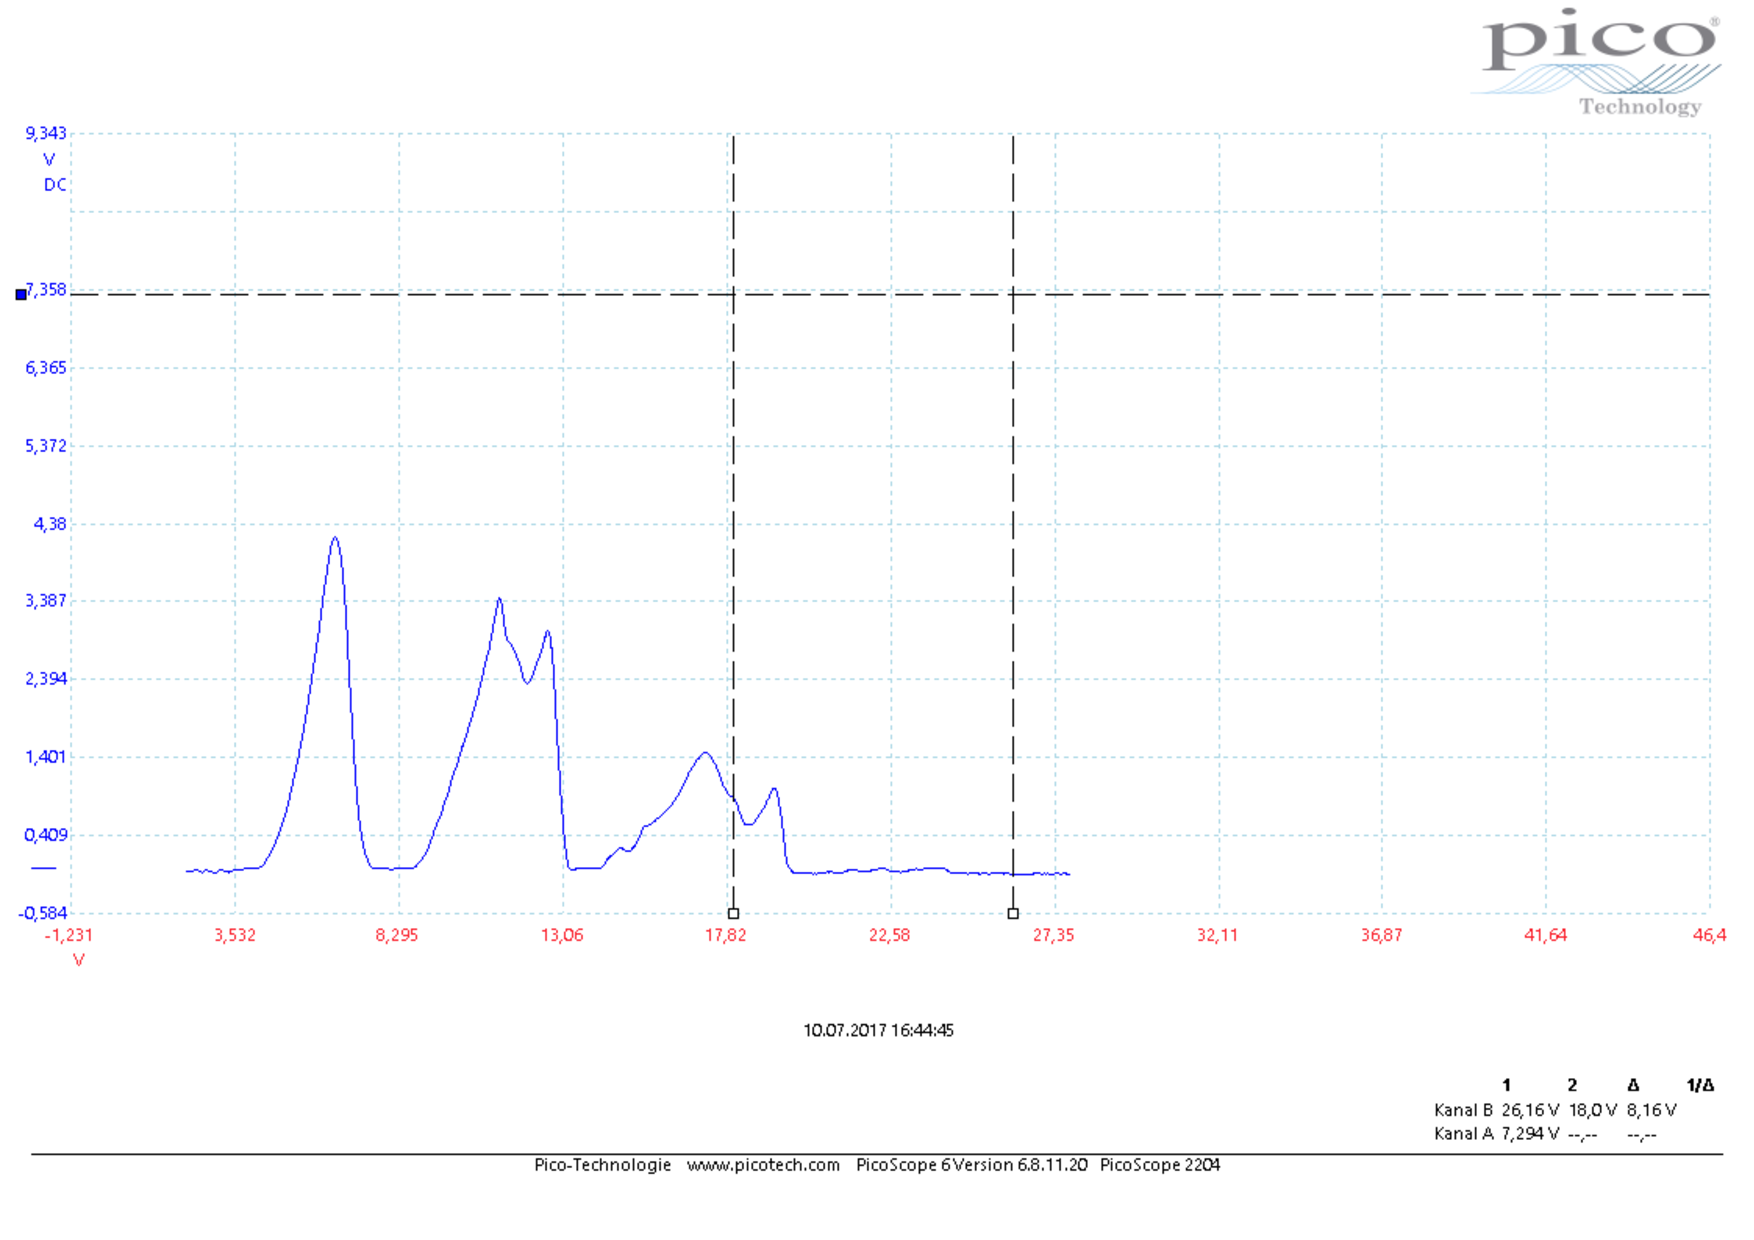
\includegraphics[width=\textwidth]{../Daten/Frank_Hertz_2.pdf}
	\caption{Frank-Hertz-Kurve mit 1. und 2. Anregung}
	\label{fig:FrankHertz2}
\end{figure}
Man sieht in dem Plot gut die Anregungen, welche Linearkombinationen der in \ref{tab:hgAnr} aufgelisteten Anregungen sind.
\begin{table}
	\centering
	\caption{Anregungsniveaus von Quecksilber}
	\begin{tabular}{l | c c}
		\toprule
		1. Anregung (a) & $6s^1S_0$ nach $6p^3P_1$ & 4,9V\\
		2. Anregung (b)& $6s^1S_0$ nach $6p^1P_1$ & 6,7V\\
	\end{tabular}
	\label{tab:hgAnr}
\end{table}
In~\ref{tab:hgAnrgem} sind die Verschiedenen Peaks mit den durch Vergleich ermittelten Anregungen aufgetragen.
An~\ref{tab:hgAnrgem} lässt sich auch gut erkennen, dass die Kurve um ca 2 V nach oben verschoben ist.
Dies kann auf eine fehlerhafte Kalibrierung des Betriebsgerätes zurückgeführt werden.
\begin{table}
	\centering
	\caption{Gemessene Anregungen von Quecksilber}
	\begin{tabular}{l | c c}
		Peak / Knick & $U_g$ in V& Anregung\\
		\midrule
		1 & 5,5 & a \\
		2 & 10,9 & 2 a \\
		3 & 12,3 & a + b \\
		4 & 14,5 & 2 b \\
		5 & 16,3 & 2 a + b \\
		6 & 19,0 & a + 2 b \\
	\end{tabular}
	\label{tab:hgAnrgem}
\end{table}
\section{Bemerkungen zur Einstellung des Versuches}
Die Einstellung des Versuches ist in kleinen schritten durchgeführt worden da der Graph bereits für Änderungen um ca. 100 mV grosse Abweichungen zeigt.
Es wurden ca. 15 Versuche gebraucht die für das Bild optimalen Einstellungen zu finden.
